\section*{Process}
Processen er bevidst opdelt i kategorier, der eksekveres med tidsmæssigt
overlap. Ideen er at starte med at skære alt massiv træ op på råmål tidligt,
samt stavlime hvor nødvendigt. Derefter udføres arbejde med pladematerialer og
finer. Udskæring på finmål af de opskårede emner udskydes til de hver i sær skal
bruges. Denne fremgang forlænger den tilgængelige tid til akklimatisering af
træet, mht. Værkstedets luftfugtighed, uden at forsinke arbejdet.

\subsection*{Skabeloner}
Udoveer diverse opstillinger, bruges der to skabeloner i projektet, begge til
benene. En skabelon bruges til tapering, og en til udfræsningen i toppen.

\begin{figure}[htb]
\centering
\fbox{
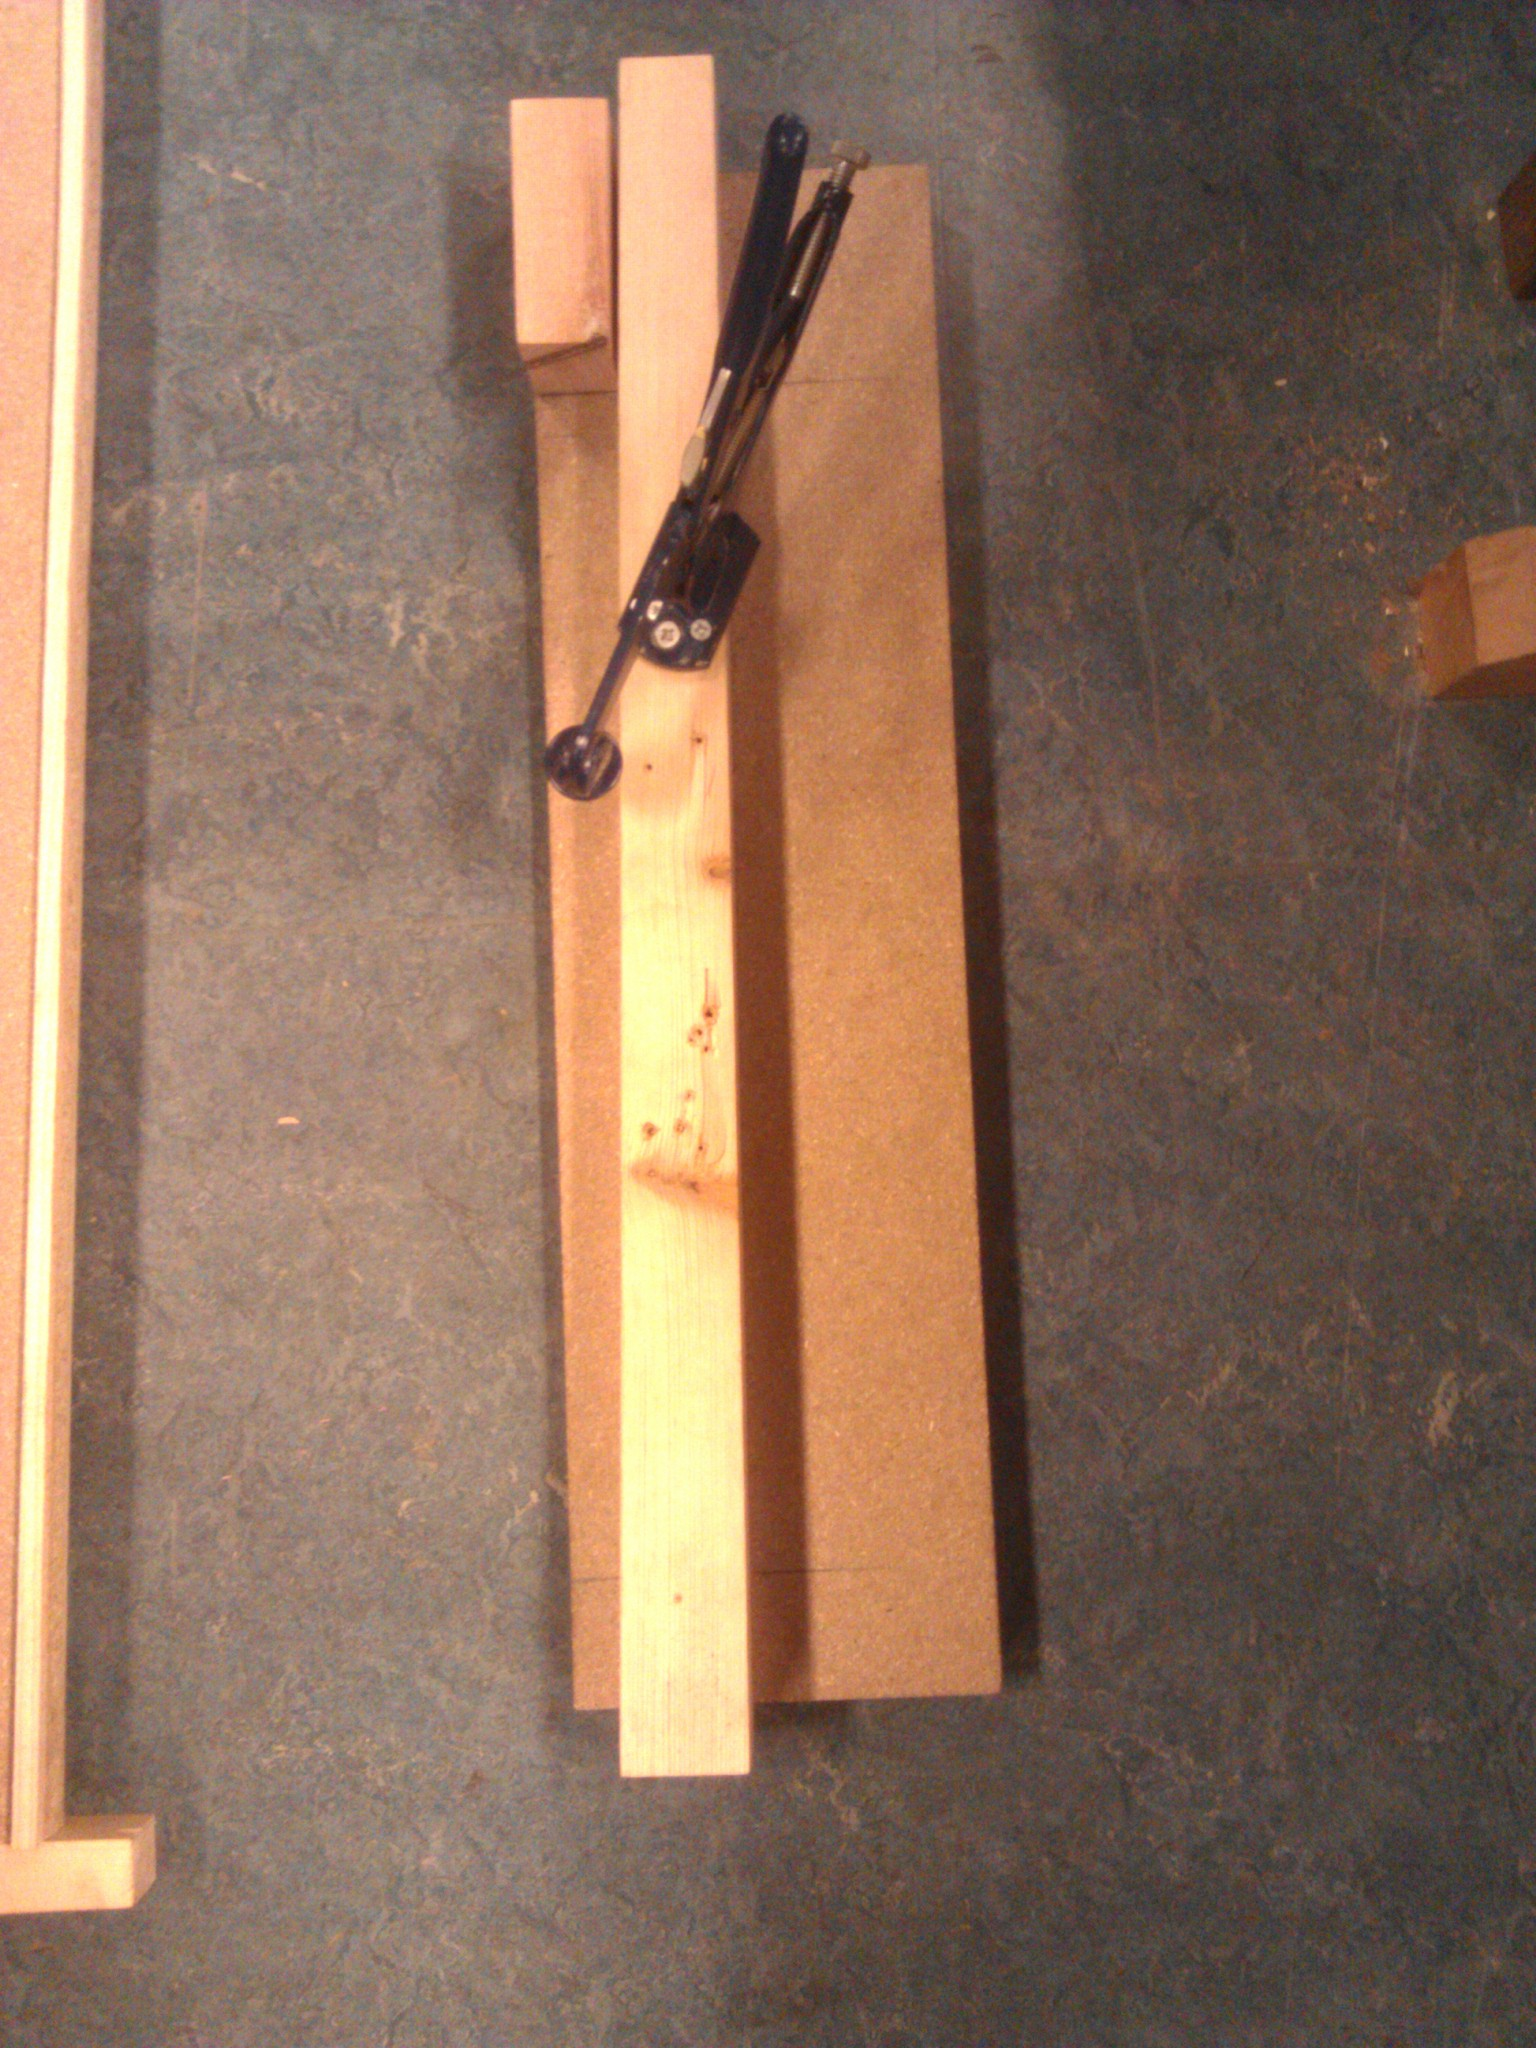
\includegraphics[width=0.4 \textwidth]{imgs/skabelon-tapering.jpg}
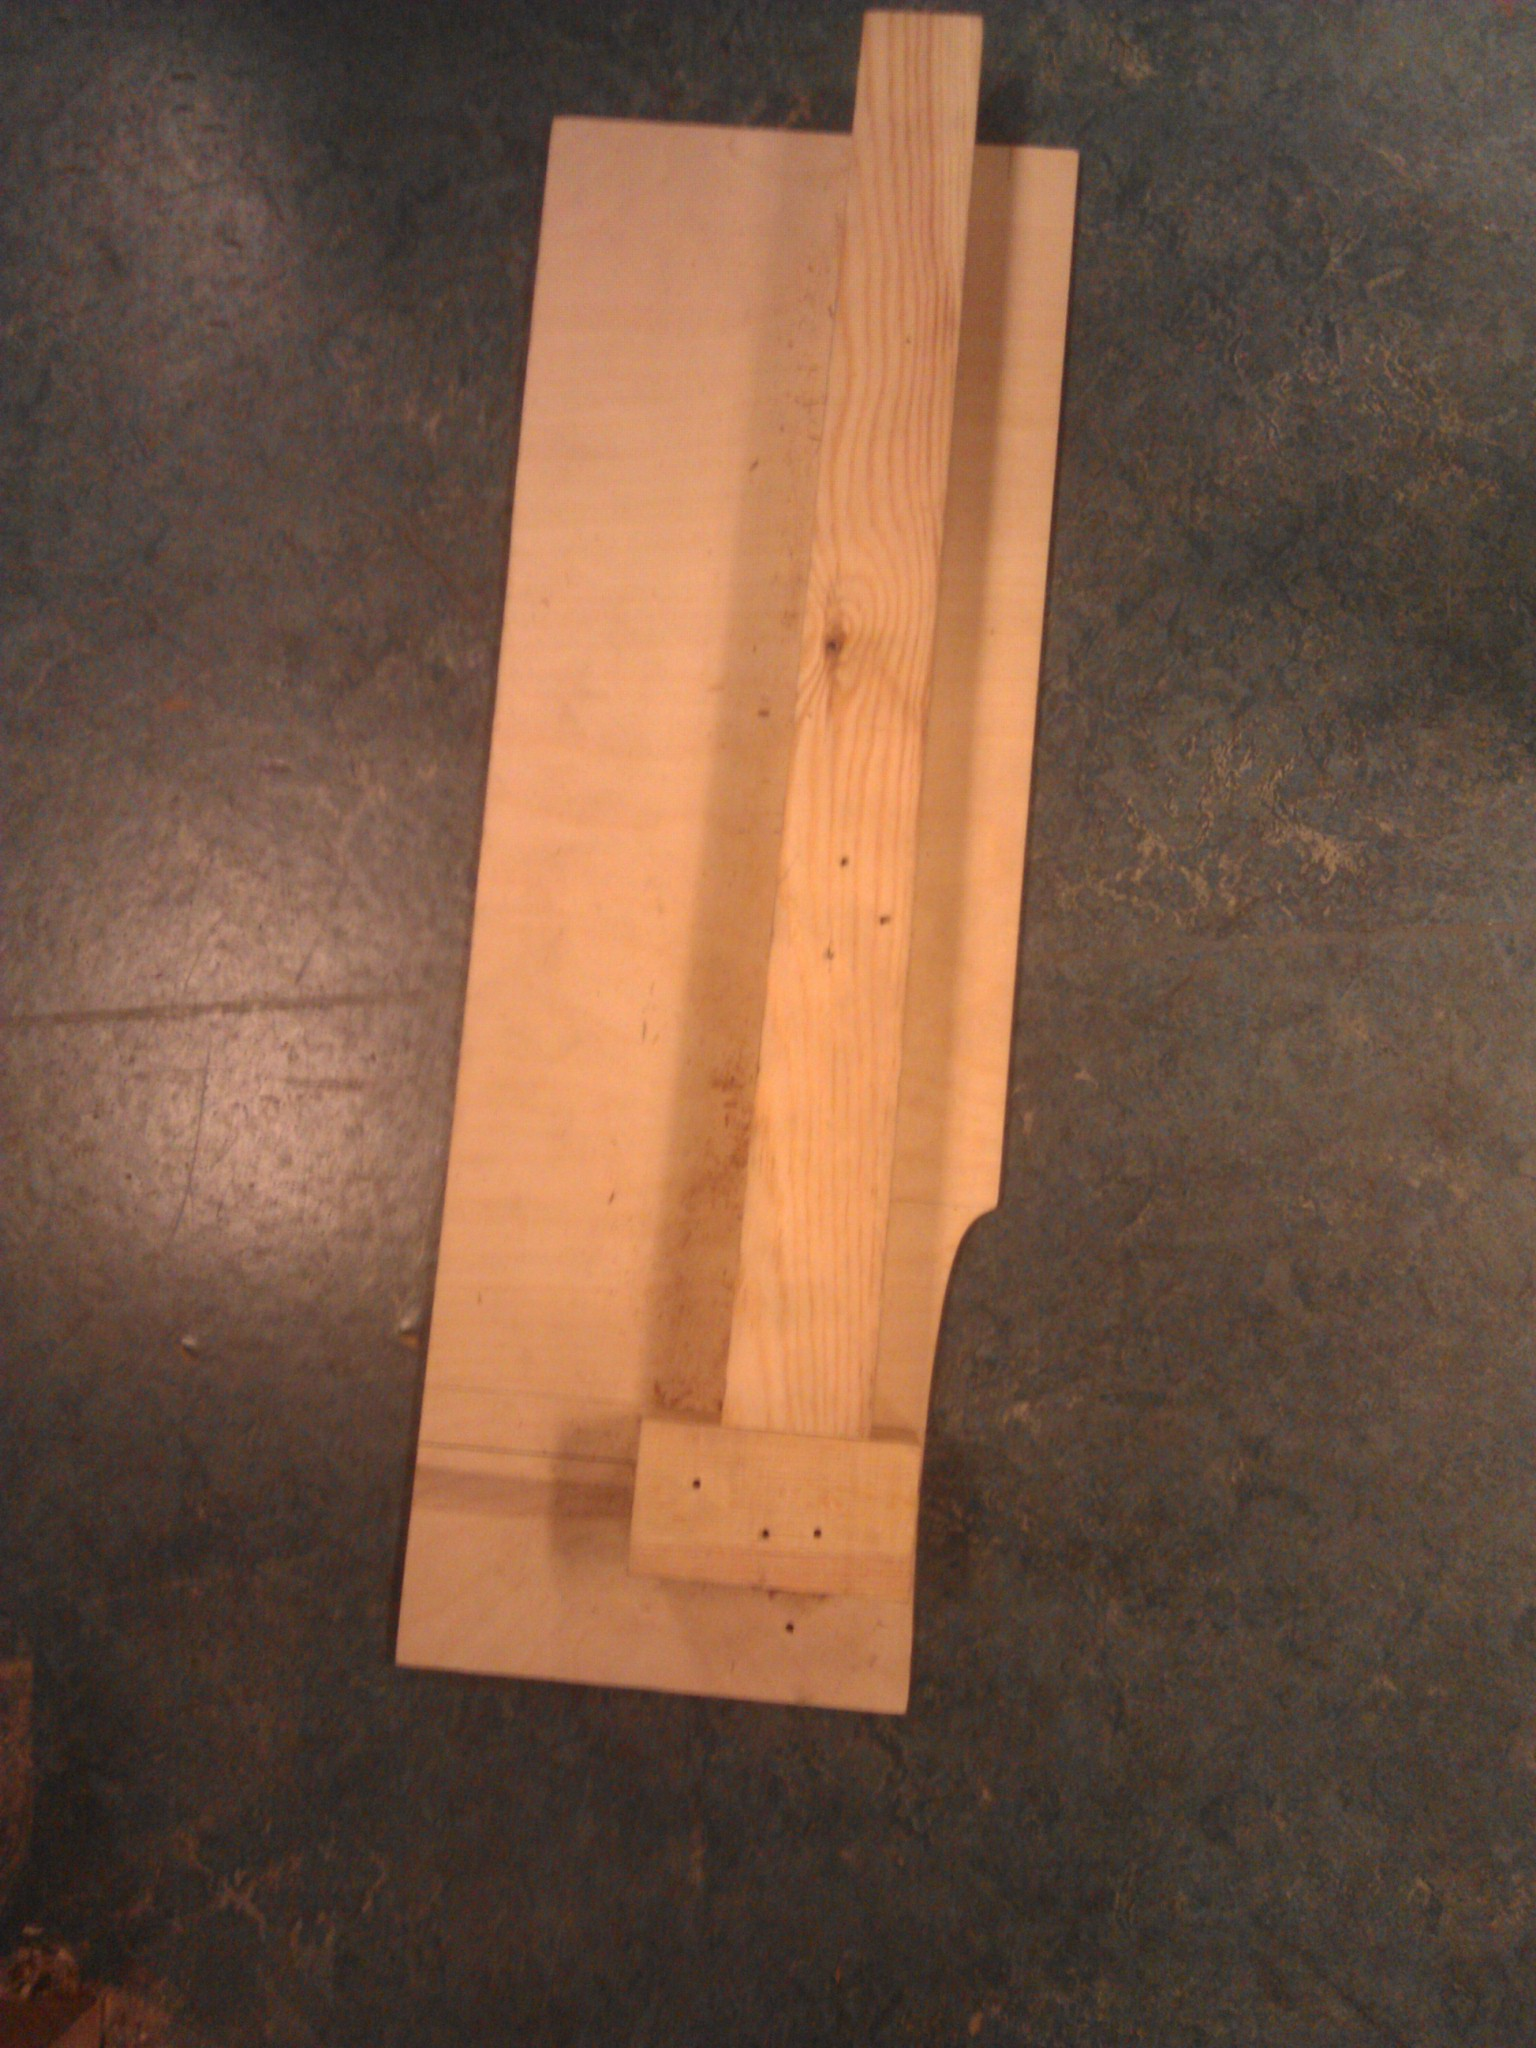
\includegraphics[width=0.4 \textwidth]{imgs/skabelon-fraesning.jpg}
}
\caption{Skabelon til tapering af ben (venstre). Skabelon til udfræsning (højre)}
\end{figure}

Taperingen udføres på formatrundsav, hvor en liste på skabelonenes underside
passer ned i en rille i fomratsavens land. Benet køres så på langs "forbi"
klingen der ligger helt tæt op af skabelonen.

Fræseskabelonen består af to land og et stop, med en udskæring fræsejernets leje kan køre
op ad. På grund af benenes tykkelse er det nødvendigt at fræse hver side to
gange. Først med et jern der har lejet ind mod fræseren, og derefter med et jern
der har lejet væk fra fra fræseren. Ved anden fræsning kan lejet køre opad
snittet fra den første fræsning.

\subsection*{Overfladebehandling}
Møblet behandles til sidst med træolie, der gør træet en smule mørkere.
Olien beskytter træet mod eksterne påvirke, og kan endda mindske påvirkningen af
variationer af luftfugtigheden. Dog kræves ekstra arbejde hvis træet skal
"lukkes" - så meget som det nu kan blive lukket.
Først pudses møblet ned, og da påføres første lag olie. Da porerne i træet vil
rejse sig som olien trækker ind i træet, pudses/slibes møblet ned mellem olie
lagene. Det er dog vigtigt at man ikke pudser for meget, da man ikke ønsker at
pudse den olierede flade bort, men blot at fjerne de oprejste porer.
